\chapter{Introduction} \label{introduction}
This chapter will introduce the problem addressed in this project. 
Previous similar projects as well as the value of this research will also be addressed.

\section{Background and Motivation}

Traditionally the thermal conductivity, otherwise referred to as the $\kappa$-value, of timber is based simply off the EN 1995:1-1-2004 or similar standards.
This research project will aim to obtain the thermal diffusivity of cross laminated SA-Pine timber by further analysing data obtained by S. van der Westhuyzen for his study of the samples' charring rate.

The thermal diffusivity of timber is a unobservable quantity that cannot be measured directly. Instead, it is related to measurements of temperature and time through differential models. 
When heat diffusion is calculated using Finite Element methods(TODO:choose which FEM), the process is usually simplified to a linear problem \citep{Fish:2007}. 
Due to the changes in thermal diffusivity of timber with temperature, as can be seen in EN 1995:1-1-2004(pg number TODO), the diffusivity cannot be linearly modelled. 
Therefore, the problem lends itself to being analysed by inversion techniques. 
The aforementioned approach will allow us to obtain information about the diffusivity based on the combination of the information assumed prior to measuring, further referred to as the prior, and the measured data. 
Using statistical inversion leads to a probability distribution that provides us with a collection of diffusivity estimates and their corresponding probabilities.

Currently the fire rating of specific timber samples are based on fire tests conducted in a furnace. 
	The furnace is kept at increasing temperatures corresponding with the Standard or ISO 834 fire curve as specified in ISO 834 \citet{ISO:1999}.
	This process becomes very costly if it has to be repeated every time that timber is used for construction, as timber usage for multiple story construction projects have increased over the past decades. 
	This increase is partially due to the sustainability of timber as a construction material: not only is it renewable but it also has a small carbon footprint \citep{Salvadori:2017}
%This will be done by adjusting a finite element model created by Dr. N de Koker into a function. This function will be used in a Bayes model to solve for the temperature dependant thermal diffusivity.
\section{Aim and objectives}
During the course of the project, the student will aim to meet the following objectives:
\begin{enumerate}
 \item Modify a Finite Element Model into an accurate and effective function;
 \item Compare the model data to the actual acquired data;
 \item Solve for the thermal diffusivity using Bayes' theorem of inverse problems; and
 \item Evaluate and explore the posterior probability distribution using the following methods:
 	\begin{enumerate}
 		\item Maximum a Posteriori
 		\item Markov-Chain Monte Carlo 	
 	\end{enumerate}
\end{enumerate}

\section{Current knowledge}
	
	
	The current $\kappa$-values used for the design of timber elements are taken from the EURO code (ref TODO \citep{Euro:2004}) and are show in figure \ref{kvalue_fig}.  
	\begin{figure}[H]
	\label{kvalue_fig}
	\centering
	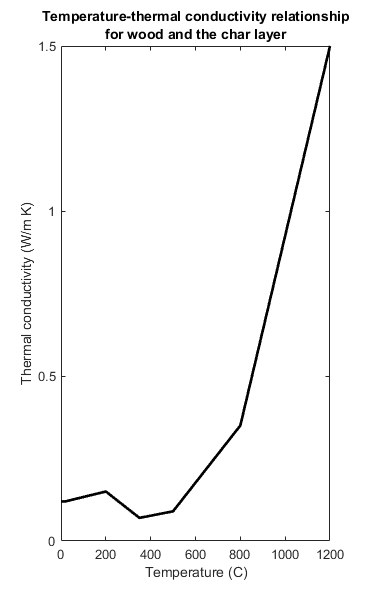
\includegraphics[width = \linewidth]{figures/kvalues_euro.png}
	\caption{Standard temperature-thermal conductivity relationship for timber from \citep{Euro:2004}}
	\end{figure}
	

	
\section{Program}